% Figure from MATH 556 notes, section 18. Compile with the notes preamble.
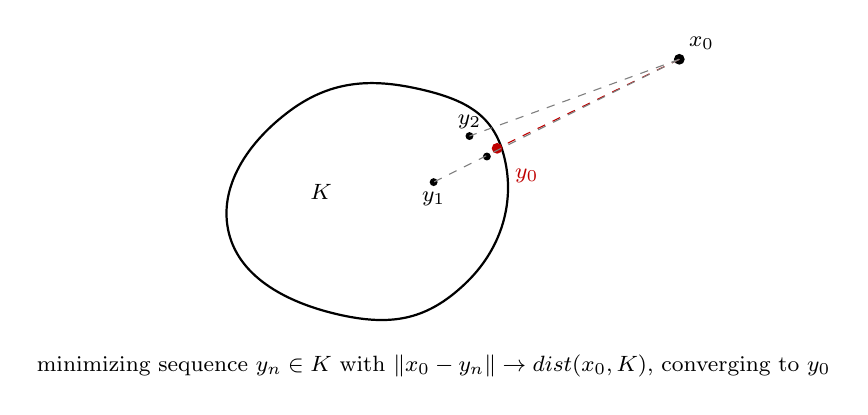
\begin{tikzpicture}[scale=1.3, >=stealth]
\draw[thick] plot[smooth cycle, tension=0.8] coordinates {(-1.4,-0.3) (-0.8,0.9) (0.5,1.1) (1.3,0.4) (0.9,-0.8) (-0.3,-1.1)};
\node[font=\footnotesize] at (-0.5,0.1) {$K$};
\fill (3.0,1.4) circle (1.5pt) node[above right, font=\footnotesize] {$x_0$};
\fill[red!75!black] (1.22,0.53) circle (1.5pt) node[below right, font=\footnotesize, xshift=3pt, yshift=-4pt] {$y_0$};
\draw[dashed, red!75!black] (3.0,1.4) -- (1.22,0.53);
\fill (0.6,0.2) circle (1.1pt) node[below, font=\footnotesize] {$y_1$};
\fill (0.95,0.65) circle (1.1pt) node[above, font=\footnotesize, yshift=-1pt] {$y_2$};
\fill (1.12,0.45) circle (1.1pt);
\draw[dashed, gray] (3.0,1.4) -- (0.6,0.2);
\draw[dashed, gray] (3.0,1.4) -- (0.95,0.65);
\node[font=\footnotesize] at (0.6,-1.6) {minimizing sequence $y_n \in K$ with $\|x_0 - y_n\| \to \operatorname{dist}(x_0, K)$, converging to $y_0$};
\end{tikzpicture}
